\documentclass{aip-cp}

\usepackage[numbers]{natbib}
\usepackage{rotating}
\usepackage{graphicx}

% Document starts
\begin{document}

% Title portion
\title{Light Meson Decays from Photon-Induced Reactions with CLAS}

\author[aff1,aff2]{Michael C. Kunkel\corref{cor1} }
\author[]{on behalf of the CLAS Collaboration }
\affil[aff1]{Forschungszentrum J\"ulich, J\"ulich (Germany)}
\affil[aff2]{Old Dominion University, Norfolk Virgina (USA)}
\corresp[cor1]{m.kunkel@fz-juelich.de}

\maketitle

\begin{abstract}
Photo-production experiments with the CEBAF Large Acceptance Spectrometer (\textsc{\texttt{CLAS}}) at the Thomas Jefferson National Laboratory produce data sets with unprecedented statistics of light mesons. With these data sets, measurements of transition form factors for $\eta$, $\omega$, and $\eta^\prime$ via conversion decays can be performed using a line shape analysis on the invariant mass of the final state dileptons. Tests of fundamental symmetries and information on the light quark mass difference can be performed using a Dalitz plot analysis of the meson decay. An overview of the first results and future prospects within the newly upgraded \textsc{\texttt{CLAS}} apparatus will be given.
\end{abstract}

% Head 1
\section{INTRODUCTION}
Decays of light mesons provide insight into the structure of the meson. The Light Meson Decay (LMD) group, established at the Thomas Jefferson National Facility with worldwide collaboration, investigates physics pertaining to, but not limited to, transition form factors, anomalous decays and the search for CP violation through Dalitz plot analysis. The presentation given was an overview of the LMD program, recent updates on measurements and an outlook on measurements that can be taken with the CLAS12 detector. 

\section{Light Meson Decay Program}
The light meson group was established in 2013. The goal of the group is to investigate properties of light meson decays using data obtained from the CLAS detector.
\begin{figure}[h]
	\centerline{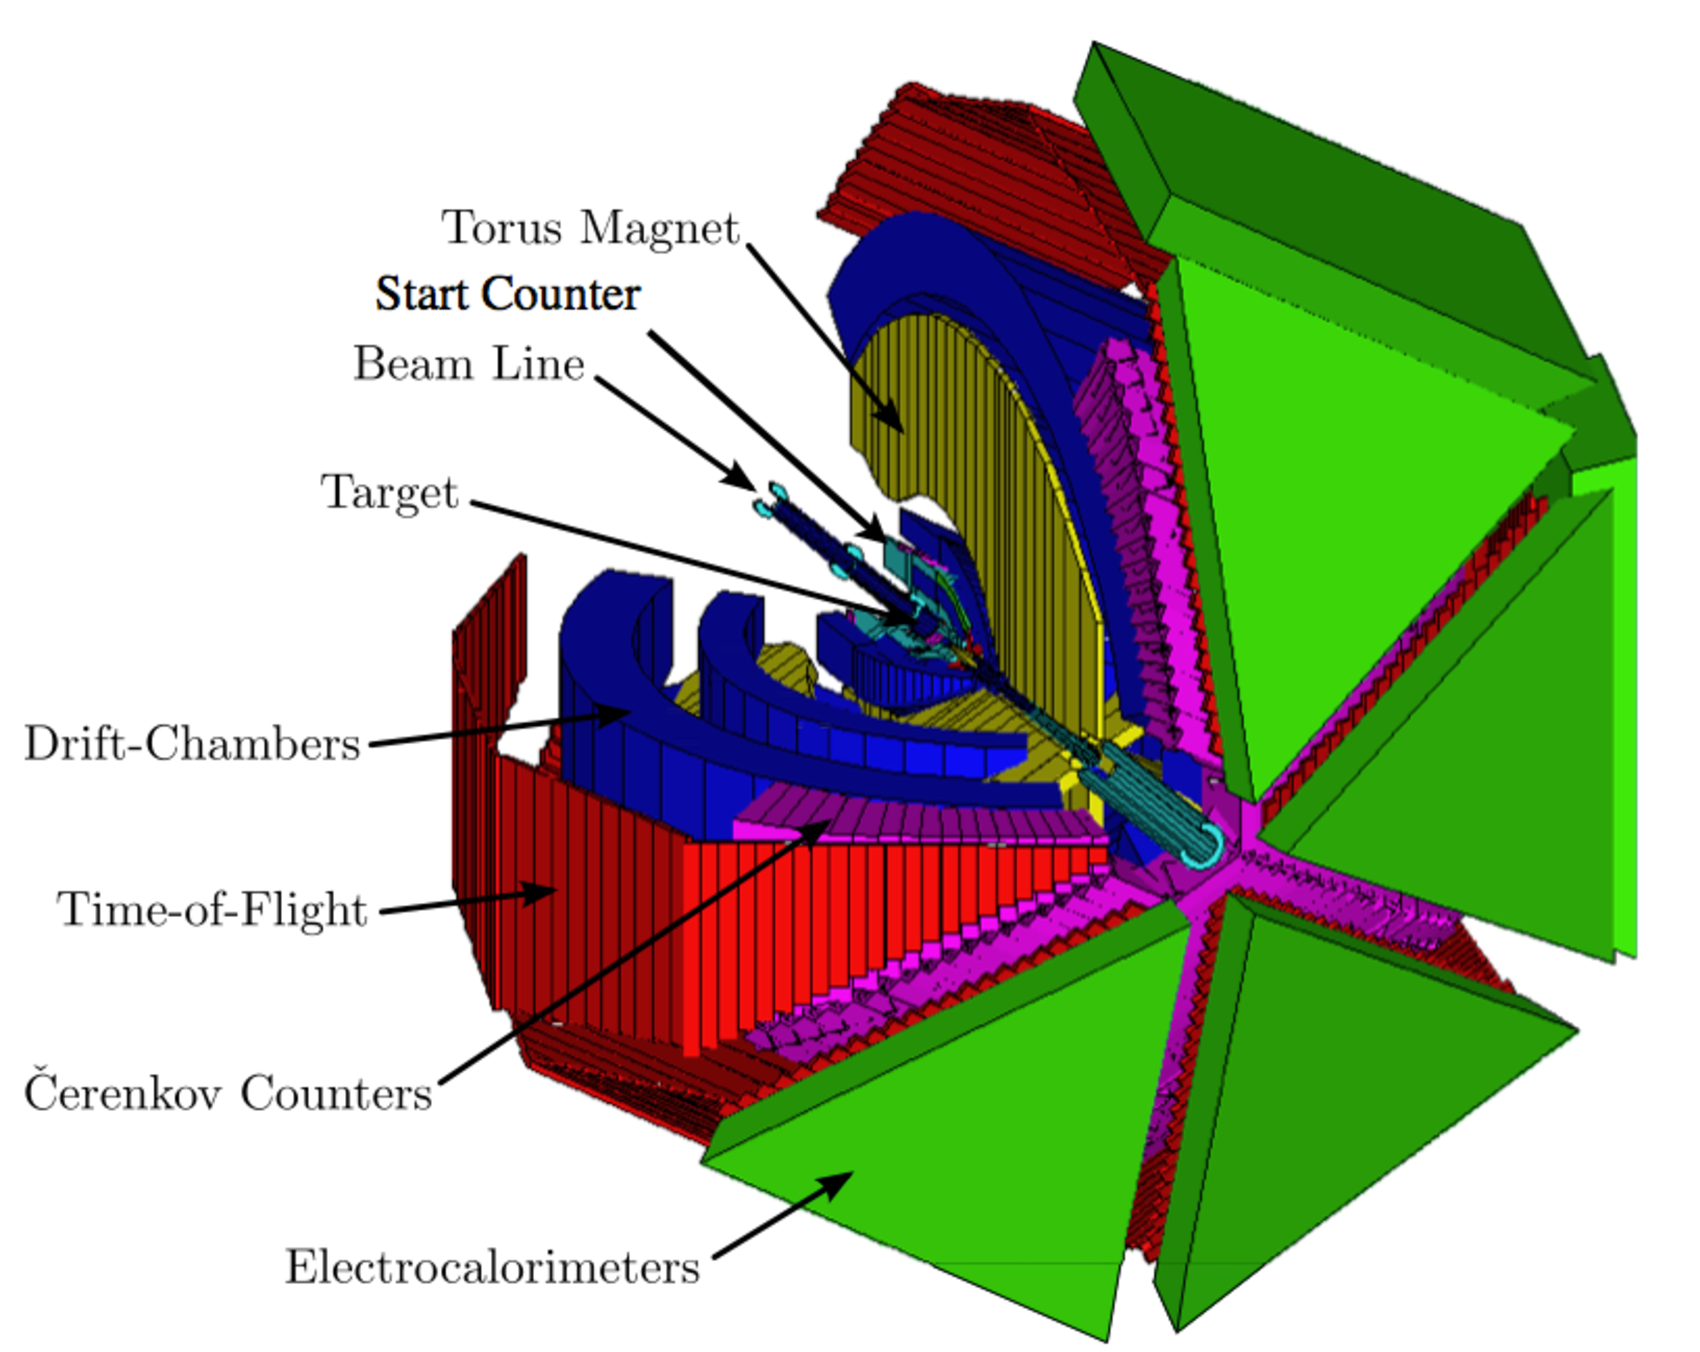
\includegraphics[width=150pt]{figures/clas_schematicIII.pdf}}
	\caption{The CEBAF Large Acceptance Spectrometer (CLAS) }
\end{figure}
 Since decays of hadrons are independent of production, all CLAS data can be used, however there are two experiments that were chosen as flagships for the program, the g11 and g12 experiment. Both experiments are use photon beam incident on a liquid hydrogen target which create photo-induced reactions 
\begin{table}[h!]
\begin{minipage}{\textwidth}
\begin{center}


\caption{\label{tab:lmd.channels}LMD planned measurements \vspace{0.75mm}}
\begin{tabular}{cc||cc}
%\begin{tabular}{p{5cm} | p{7cm}}
\hline
Meson Decay & Physics Interest &Meson Decay & Physics Interest \\
\hline
$\pi^0\to e^+e^-\gamma$  & Heavy photon upper limit &$\eta^{\prime}\to \pi^+\pi^-\gamma$  & Box anomaly \\
$\eta^{\prime}\to e^+e^-\gamma$  & Transition form factor &$\omega\to \pi^+\pi^-\gamma$  & Upper limit branching ratio \\
$\omega\to e^+e^-\pi^0$ & Transition form factor & $\eta, \omega, \phi\to \pi^+\pi^-\pi^0$ & Dalitz plot analysis\\
$\eta^{\prime}\to e^+e^-\pi^0$ & C violation & $\eta^{\prime}\to \pi^+\pi^-\eta$ & Dalitz plot analysis\\
$\eta^{\prime}\to e^+e^-\pi^+\pi^-$  & CP violation & $\phi\to \pi^+\pi^-\eta$ & G-parity violation\\
\hline 
\end{tabular}


\end{center}
\end{minipage}
\end{table}
\vspace{20pt}
\subsection{Update on the Radiative decay of the $\eta$ meson}

\subsection{Update on the Dalitz Plot anlaysis of the $\eta^\prime$ meson}

\subsection{Update on the transistion form factor measurement  of the $\omega$ meson}

\subsection{Update on the branching ratio measurement  of the $\eta^\prime$ meson $\rightarrow e^+e^-\gamma$}
\subsection{Future measurement of the $\eta^\prime$ meson transsition form factor with CLAS12}

% Acknowledgement
\section{ACKNOWLEDGMENTS}
The reference section will follow the ``Acknowledgment'' section.  References should be numbered using Arabic numerals followed by a period (.) as shown below, and should follow the format in the below examples.

% References

\nocite{*}
\bibliographystyle{aipnum-cp}%
\bibliography{sample}%


\end{document}
